\documentclass{standalone}
\usepackage{pgfplots}
\usepackage{tikz}
\usetikzlibrary{automata}
\usetikzlibrary {positioning}
\usepackage{raha_tikz}

\begin{document}
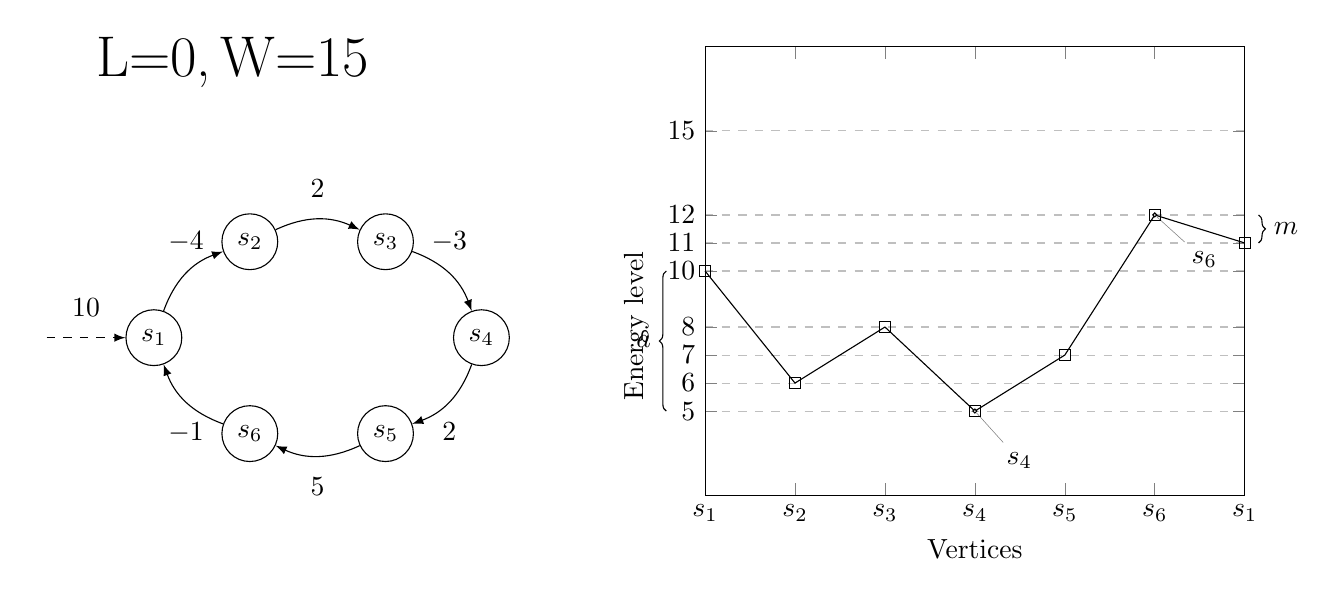
\begin{tikzpicture}[scale=1,auto ,node distance =1 cm,
state/.style ={ circle,draw}]
    \begin{scope}[yshift=-2cm]
    \node[state] (A) [] {$s_1$};
\node[state] (B) [above right=of A] {$s_2$};
\node[state] (C) [right=of B] {$s_3$};
\node[state] (D) [below right=of C] {$s_4$};
\node[state] (E) [ below left=of D] {$s_5$};
\node[state] (F) [left=of E] {$s_6$};
\node (01) [left =of A] {$$};
\path (1,3.5) node[text width=4cm,align=center] { \huge L=0, W=15};

\path (01) edge [-latex,dashed] node[above =0.15 cm] {$10$} (A);
\path (A) edge [-latex,bend left =25] node[above =0.15 cm] {$-4$} (B);
\path (B) edge [-latex,bend left =25] node[above =0.15 cm] {$2$} (C);
\path (C) edge [-latex,bend left =25] node[above =0.15 cm] {$-3$} (D);
\path (D) edge [-latex,bend left =25] node[below =0.15 cm] {$2$} (E);
\path (E) edge [-latex,bend left =25] node[below =0.15 cm] {$5$} (F);
\path (F) edge [-latex,bend left =25] node[below =0.15 cm] {$-1$} (A);
    \end{scope}
%
    \begin{scope}[xshift=7cm, yshift=-4cm]
    \begin{axis}[
    title={},
    xlabel={Vertices},
    ylabel style= {xshift=-20pt},
    ylabel={ Energy level},
    clip=false,
    xmin=1, xmax=7,
    ymin=2, ymax=18,
    xtick={1,2,3,4,5,6,7},
    ytick={5,6,7,8,10,11,12,15},
    xticklabels={$s_1$,$s_2$,$s_3$,$s_4$,$s_5$,$s_6$,$s_1$},
     legend pos=north east,
    ymajorgrids=true,
    grid style=dashed,
]

\addplot[
    color=black,
    mark=square,
    ]
    coordinates {
    (1,10)(2,6)(3,8)(4,5)(5,7)(6,12)(7,11)
    }; 

\node[inner sep=0.5pt,circle,draw,-latex,fill=white,pin=-55: $s_4$] 
	  at (axis cs:4,5) {};
	  \node[inner sep=0.5pt,circle,draw,-latex,fill=white,pin=-45: $s_6$] 
	  at (axis cs:6,12) {};


\draw[decorate,decoration={brace}]
  ([xshift=-14pt]axis cs:1,5) --
    node[left=2pt] { $a$} 
  ([xshift=-14pt]axis cs:1,10);

\draw[decorate,decoration={brace,mirror}]
  ([xshift=5pt]axis cs:7,11) --
    node[right=2pt] {$m$} 
  ([xshift=5pt]axis cs:7,12);
\end{axis}
      \end{scope}
  \end{tikzpicture}
\end{document}
